\begin{center}
\Huge
Cirkler og linjer
\end{center}

\section*{Skæring mellem cirkel og linje}
\stepcounter{section}
Vi skal afgøre, hvordan vi bestemmer skæringspunkter mellem cirkler og linjer. Vi ser derfor på et eksempel.
\begin{exa}
	Lad os betragte en cirkel $C$ med centrum i $(4,2)$ og radius 8. Denne 
	cirkel har ligningen 
	\begin{align*}
		(x-4)^2 + (y-2)^2 = 64.
	\end{align*}
	Lad os desuden betragte en linje $l$ med ligningen
	\begin{align*}
		l: \ 2(x-1) -2(y-3) = 0. 
	\end{align*}
	Disse kan ses på Figur \ref{fig:cirkellinje}.
	\begin{figure}[H]
		\centering
		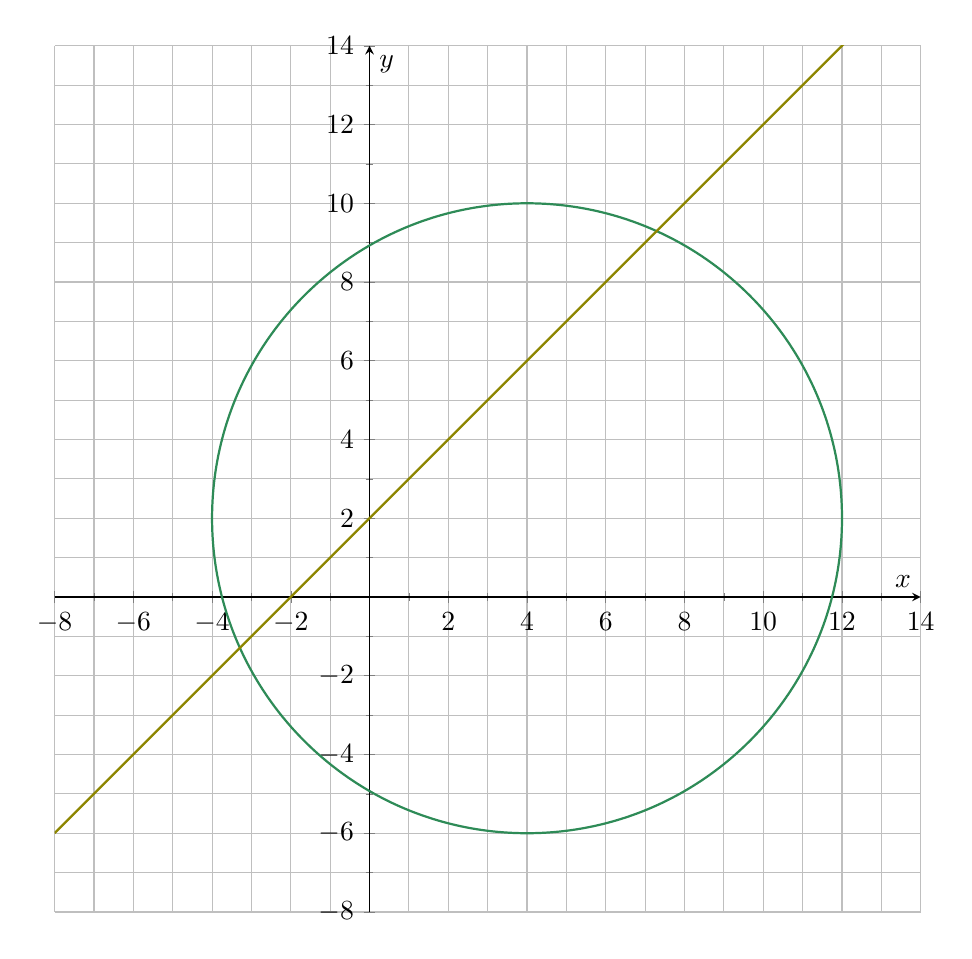
\begin{tikzpicture}
		\begin{axis}
			[
			axis lines = center, 
			x = 0.5cm, y = 0.5cm,
			xmin = -8, xmax = 14, 
			ymin =-8, ymax = 14,
			grid = both,
			minor tick num = 1, 
			xlabel = $x$, ylabel = $y$,
			]	
			\draw[color = SeaGreen, thick] (axis cs: 4,2) circle (4cm); 
			\addplot[color = olive, thick, domain = -8:14] {2 + x}; 
		\end{axis}		
		\end{tikzpicture}
		\caption{Cirklen $C$ og linjen $l$.}
		\label{fig:cirkellinje}
	\end{figure}
	Vi bestemmer skæringspunktet mellem disse i Maple. Dette gøres ved at skrive følgende kommando. 
	\begin{align*}
		&\texttt{restart}\\
		&\texttt{with(Gym):}\\
		&\texttt{l:= 2(x-1) - 2(y-3) = 0}\\
		&\texttt{C:=(x-4)$^\texttt{2}$ + (y-2)$^\texttt{2}$ = 64}\\
		&\texttt{solve([C,l])}\\
	\end{align*}
	Vi kan bestemme skæringspunkterne mellem disse i Maple. De bestemmes til at være $(-3.3, -1.3)$ og $(7.3,9.3)$. 
\end{exa}

\section*{Tangent til cirkel}
\stepcounter{section}

En tangent til en cirkel er en ret linje, der følger langs en cirkel og som rører cirklen i netop ét punkt. Kender vi centrum til en cirkel samt et punkt, hvor vi ønsker en tangent, så kan vi bestemme en tangent til cirklen i lige netop det punkt. Lad os betragte et eksempel. Idéen kan ses på Figur \ref{fig:cirkeltangent}.
\begin{figure}[H]
	\centering
	\begin{tikzpicture}
		\begin{axis}[axis lines = middle, 
		ticks = none,
		xmin = -2, xmax = 8,
		ymin = -2, ymax = 8,
		x = 0.8cm, y = 0.8cm,
		xlabel = $x$, ylabel = $y$,]
			\draw[thick, color = olive] (axis cs: 2,3) circle[radius = 4];
			\addplot[color = teal, thick, domain = -2:8] {-0.849*x+9.964};
			\filldraw[color = olive] (axis cs: 2,3) circle[radius =2pt];
			\draw[-{Stealth[scale = 1.3]}, thick, color = teal] (axis cs: 4.59,6.05) to (axis cs:2,3);
		\end{axis}
	\end{tikzpicture}
	\caption{Tangent til cirkel.}
	\label{fig:cirkeltangent}
\end{figure}
\begin{exa}
	En cirkel med centrum i $C(3,5)$ og radius $5$ er givet. Punktet $P(7, 8)$ ligger på cirklen.
	Vi skal bestemme ligningen for tangenten til cirklen, der går gennem dette punkt. En normalvektor må være givet som
	forbindelsesvektoren mellem centrum for cirklen og punktet $P$ på randen af cirklen, som vi kan se på Figur
	 \ref{fig:cirkeltangent}. Denne bestemmes altså som
	\begin{align*}
		\vv{PC} = 
		\begin{pmatrix}
			x_1 - x_0 \\
			y_1 - y_0
		\end{pmatrix} 
		=
		\begin{pmatrix} 
			3 - 7 \\
			5 - 8
		\end{pmatrix}
		=
		\begin{pmatrix}
			-4 \\
			-3
		\end{pmatrix}
	\end{align*}
	Desuden går tangentlinjen selvfølgelig igennem punktet $P$. Derfor kan vi indsætte dette i cirklens ligning
	\begin{align*}
		a(x-x_0) + b(y-y_0)=0,
	\end{align*}
	og vi får
	\begin{align*}
		-4(x-7) -3(y-8) = 0
	\end{align*}
	som tangentens ligning. 
	Vi kan tegne situationen. Dette ses på Figur \ref{fig:ctexa}.
	\begin{figure}[H]
		\centering
		\begin{tikzpicture}
		\begin{axis}
		[
		axis lines = center, 
		xmin = -4, ymin = -2,
		xmax = 10, ymax = 12,
		y = 0.7cm, x = 0.7cm,
		grid = both, 
		minor tick num = 1,  
		]
			\addplot[color = olive, thick, domain = -4:10] {-4/3*x + 52/3};				
			\draw[thick, color = teal] (axis cs: 3,5) circle ({5*0.7cm});
			\filldraw[color = SeaGreen] (axis cs: 3,5) circle (2pt);
			\node[color = SeaGreen, anchor = north east] at (axis cs: 3,5) {$C$};
			\node[color = SeaGreen, anchor = south west] at (axis cs: 7,8) {$P$}; 
			\filldraw[color = SeaGreen] (axis cs: 7,8) circle (2pt);
			\draw[-{Stealth[scale = 1.3]}, thick, color = SeaGreen] (axis cs: 7,8) -- (axis cs: 3,5)
			node[midway, anchor = north west] {$\vv{PC}$};
		\end{axis}
		\end{tikzpicture}
		\caption{Eksempel på tangent til cirkel.}
		\label{fig:ctexa}
	\end{figure}
\end{exa}
Vi kan også bestemme skæringspunkter mellem cirkler og linjer uden brug af CAS-værktøj. Dette giver os typisk en andengradsligning, vi kan løse.
\begin{exa}
	Vi ønsker at bestemme skæringspunktet mellem cirklen $c$ og linjen $l$ givet ved henholdsvis
	\begin{align*}
		&c: \ (x - 4)^2 + (y - 2)^2 = 25,\\
		&l: \ y = \frac{1}{3}x - 1.
	\end{align*}
\end{exa}
Vi indsætter udtrykket for $y$ i den øverste ligning og får
\begin{align*}
	(x-4)^2 + (y - 2)^2 = 25 \ &\Leftrightarrow \ (x-4)^2 + (\frac{1}{3}x-1-2)^2 = 25 \\
	&\Leftrightarrow \ x^2 + 16 - 8x + \frac{1}{9}x^2 + 9 - 2x = 25 \\
	&\Leftrightarrow \ \frac{10}{9}x^2 + 25 - 10x = 25 \\
	&\Leftrightarrow	\ \frac{10}{9}x^2 -10x = 0 \\
	&\Leftrightarrow \ x\left(\frac{10}{9}x - 10\right) = 0 \\
\end{align*}
Derfor er $x = 0$ eller $\frac{10}{9}x  - 10 = 0$. Dette giver
\begin{align*}
	\frac{10}{9}x - 10 = 0 \ &\Leftrightarrow \ \frac{10}{9}x = 10 \\
	&\Leftrightarrow	 \ 10x = 90 \\
	&\Leftrightarrow \ x = 9.
\end{align*} 
Derfor er $x = 0$ eller $x = 9$. For at finde $y$-værdierne i skæringspunkterne sættes disse tal ind i linjens ligning. 
\begin{align*}
	y = \frac{1}{3}\cdot 0 - 1 = -1
\end{align*}
og
\begin{align*}
	y = \frac{1}{3} \cdot 9 - 1 = 2.
\end{align*}
Skæringspunkterne mellem cirklen og linjen er derfor $(0,-1)$ og $(9,2)$. 

\subsection*{Opgave 1 (Med hjælpemidler)}
\begin{enumerate}[label=\roman*)]
	\item En cirkel $c$ og en linje $l$ er givet ved følgende ligninger:
	\begin{align*}
		&c: \ (x+2)^2+(y-2)^2 = 4, \\
		&l: \ y = -x.
	\end{align*}
	Bestem skæringspunkterne mellem $c$ og $l$. 
	\item En cirkel $c$ og en linje $l$ er givet ved følgende ligninger:
	\begin{align*}
		&c: \ x^2+(y-3)^2 = 16, \\
		&l: \ x-2 - 2(y-1) = 0.
	\end{align*}
	Bestem skæringspunkterne mellem $c$ og $l$. 
	\item En cirkel $c$ og en linje $l$ er givet ved følgende ligninger:
	\begin{align*}
		&c: \ x^2+2x+y^2+4y = 4, \\
		&l: \ 4(x+3)+3(y+3)=0.
	\end{align*}
	Bestem skæringspunkterne mellem $c$ og $l$. 
	\item En cirkel $c$ og en linje $l$ er givet ved følgende ligninger:
	\begin{align*}
		&c: \ x^2+y^2=1, \\
		&l: \ y=1.
	\end{align*}
	Bestem skæringspunkterne mellem $c$ og $l$.
\end{enumerate}

\subsection*{Opgave 2}
En cirkel $c$ har centrum i $C(-8,1)$ og punktet $P(-3,13)$ ligger på randen af cirklen.
\begin{enumerate}[label=\roman*)]
	\item Bestem ligningen for tangenten til cirklen $c$.
	\item Bestem radius af cirklen $c$. 
	\item Bestem ligningen for cirklen $c$. 
\end{enumerate}

\subsection*{Opgave 3}
En cirkel $c$ har centrum i $C(7,12)$ og punktet $P(1,20)$ ligger på randen af cirklen.
\begin{enumerate}[label=\roman*)]
	\item Bestem ligningen for tangenten til cirklen $c$.
	\item Bestem radius af cirklen $c$. 
	\item Bestem ligningen for cirklen $c$. 
\end{enumerate}

\subsection*{Opgave 4 (Med hjælpemidler)}
\begin{enumerate}[label=\roman*)]
	\item En cirkel har centrum i $(-5,4)$ og radius $3$, og en linje har ligningen $y = 2x+10$. Bestem skæringspunkterne mellem cirklen og ligningen
	\item En cirkel har ligningen $(x+2)^2+(y-7)^2 = 100$ og en linje har normalvektoren 
	\begin{align*}
		\vv{n} =
		\begin{pmatrix}
			2 \\ 1
		\end{pmatrix}
	\end{align*}
	og går gennem punktet $(-5,4)$. Bestem skæringspunkterne mellem cirklen og linjen. 
	\item En cirkel har centrum i $(1,1)$ og radius $2$, og en linje har normalvektor 
	\begin{align*}
		\vv{n} =
		\begin{pmatrix}
			-4 \\ -7			
		\end{pmatrix}
	\end{align*}
	og går gennem punktet $(1,3)$. Bestem skæringspunkterne mellem cirklen og linjen
\end{enumerate}

\subsection*{Opgave 5}
\begin{enumerate}[label=\roman*)]
	\item	En cirkel er givet ved ligningen 
	\begin{align*}
		(x-2)^2 + (y-3)^2 = 100
	\end{align*} og punktet $(6,-5)$ ligger på cirklen. Bestem ligningen for tangenten til cirklen gennem dette punkt.
	\item	En cirkel er givet ved ligningen
	\begin{align*}
		(x+1)^2 + (y+2)^2 = 25
	\end{align*}  og punktet	 $(3,1)$ ligger på cirklen. Bestem ligningen for tangenten til cirklen gennem dette punkt.	
	\item	En cirkel har centrum i $(-3,6)$ og punktet $(-10,9)$
	ligger på cirklen. Bestem ligningen for tangenten til cirklen gennem dette punkt.	
	\item	En cirkel er givet ved ligningen $x^2-4x+y^2-8y=16$ og punktet
	 $(4.70,-1.36)$
	ligger på cirklen. Bestem ligningen for tangenten til cirklen gennem dette punkt.	
\end{enumerate}

\subsection*{Opgave 6}
En cirkel $c$ har centrum i $(1,1)$ og radius $5$ og en linje $l$ er givet ved ligningen
\begin{align*}
	y = 2x + 4.
\end{align*}
\begin{enumerate}[label=\roman*)]
	\item Bestem skæringspunktet mellem $c$ og $l$ uden brug af Maple. 
\end{enumerate}

\subsection*{Opgave 7 (Med hjælpemidler)}
\begin{enumerate}[label=\roman*)]
	\item En cirkel har centrum i $(2,y_0)$ og radius $5$. Bestem tallet $y_0$, så linjen $2(x-2) + 4(y-1) = 0$ 
	er tangent til cirklen.
	\item En cirkel har centrum i $(5,4)$ og radius $7$. Bestem tallet $k$, så linjen $-6(x-k)-9(y+3) = 0$ er 
	tangent til cirklen.
	\item En cirken har centrum i $(7,1)$. Bestem radius for cirklen, så linjen $-2(x+3)-5(y-11)$ er tangent
	til cirklen. 
\end{enumerate}
